\documentclass[12pt]{article}
\usepackage[swedish,english]{babel}
\usepackage[utf8x]{inputenc}
\usepackage{amsmath}
\usepackage{graphicx}
\usepackage{float} %for insert graph
\usepackage{lscape}
\usepackage{rotating}
\usepackage[colorinlistoftodos]{todonotes}
%\usepackage[margin=1in]{geometry} %set page margin
\usepackage[bottom=1.25in, top=1.25in]{geometry}
%\addtolength{\topmargin}{0.25in}
%\addtolength{\bottommargin}{0.25in}
\usepackage{hyperref} %insert to link to email address
\usepackage{setspace}
\setlength\parindent{24pt} %set indentation
\usepackage{amssymb} %for maths symbols
\usepackage{cases} %for numbering in cases
  %define matlab style
\usepackage{listings}
\usepackage{color} %red, green, blue, yellow, cyan, magenta, black, white
\definecolor{mygreen}{RGB}{28,172,0} % color values Red, Green, Blue
\definecolor{mylilas}{RGB}{170,55,241}

\lstset{language=Matlab,%
    %basicstyle=\color{red},
    breaklines=true,%
    morekeywords={matlab2tikz},
    keywordstyle=\color{blue},%
    morekeywords=[2]{1}, keywordstyle=[2]{\color{black}},
    identifierstyle=\color{black},%
    stringstyle=\color{mylilas},
    commentstyle=\color{mygreen},%
    showstringspaces=false,%without this there will be a symbol in the places where there is a space
    numbers=left,%
    numberstyle={\tiny \color{black}}% size of the numbers
    %numbersep=9pt, % this defines how far the numbers are from the text
    %emph=[1]{for,end,break},emphstyle=[1]\color{red}, %some words to emphasise
    %emph=[2]{word1,word2}, emphstyle=[2]{style},    
}


\begin{document}

%%%%%%%%%%%
%%TITLE PAGE%%%
%%%%%%%%%%%%
\begin{titlepage}

\newcommand{\HRule}{\rule{\linewidth}{0.5mm}} % Defines a new command for the horizontal lines, change thickness here

\center % Center everything on the page
 
%----------------------------------------------------------------------------------------
%   HEADING SECTIONS
%----------------------------------------------------------------------------------------
%Logo First
%----------------------------------------------------------------------------------------
%   LOGO SECTION
%----------------------------------------------------------------------------------------


\includegraphics{UU_logo.eps}\\[0.5cm] % Include a department/university logo - this will require the graphicx package
 
\textsc{\Large Modelling complex systems}\\[0.5cm] % Major heading such as course name


%----------------------------------------------------------------------------------------
%   TITLE SECTION
%----------------------------------------------------------------------------------------

\HRule \\[0.4cm]
{\huge \bfseries Project 1: \par A firing brain \& Spread of memes }\\[0.4cm] % Title of your document
\HRule \\[1.5cm]
 
%----------------------------------------------------------------------------------------
%   AUTHOR SECTION
%----------------------------------------------------------------------------------------

{\huge Peili Guo\\} %insert your name 
{\large \href{mailto:Peili.Guo.7645@student.uu.se}{Peili.Guo.7645@student.uu.se}}
\\[2cm] %insert page break length

%----------------------------------------------------------------------------------------
%   DATE SECTION
%----------------------------------------------------------------------------------------

{\Large \today}\\[2cm] % Date, change the \today to a set date if you want to be precise


%----------------------------------------------------------------------------------------

\vfill % Fill the rest of the page with whitespace

\end{titlepage}

\newpage
%%%%%%%%%%%%
%%%start report 
%%%1. fire brain
%%%%%%%%%%%

\section{A firing brain}
\doublespacing
In this part, a simple program in matlab was written to simulate a firing brain with two-dimensional cellular automata model on a N by N grid with periodic boundary conditions.\par

each grid represents a neuron. there are 3 different states for neuron: ready(0), firing(1), and resting(2). 
the rules for transit to the next time steps are:

\begin{enumerate}
\item a ready neuron fires on the next time step if there are exactly two neighbours that are firing. ( 0 $\rightarrow$ 1, if two neighbours are 1).
\item a firing neuron goes to the resting state on the next time step (1 $\rightarrow$ 2).
\item a firing neuron goes to ready state on the next time step (2 $\rightarrow$ 0).
\end{enumerate}


\subsection{simple simulation in matlab}

Below are the results for a 40 x 40 grid where initially each cell has a probability of 0.3 being a firing(1) cell and all other neurons are ready. the figures below shows how the cells looks like after 10, 20, 100 and 1000 time steps. 

The initial probability of being in a firing state is 0.3, which means at t = 0, there are around 480 cells that are being in a firing state. as we can see in figure \ref{fig:100sim}, the total number of firing cell decreases over time. In the beginning, the number of cell decreases very fast, and the total number of cells gets stable around t = 300~400. When simulate 100 times to t = 1000, the average firing cell at t = 400 is around 14 and at t = 1000, the average firing cell is around 12. At the equilibrium state, the shapes that remains are travelling forward at a constant rate preserving the same shape either in the same direction(up/down or left/right), or will never interact if there are shape that travel in the up/down direction and others in left/right direction. Over 100 simulation, the curve of average firing cell decreases in an exponential model, and a exponential model of y = a* exp(b*x) + c*exp(d*x) was fitted to the curve in figure \ref{fig:sim_model}.


\begin{figure}[H] %figure 1 at t=10
\centering
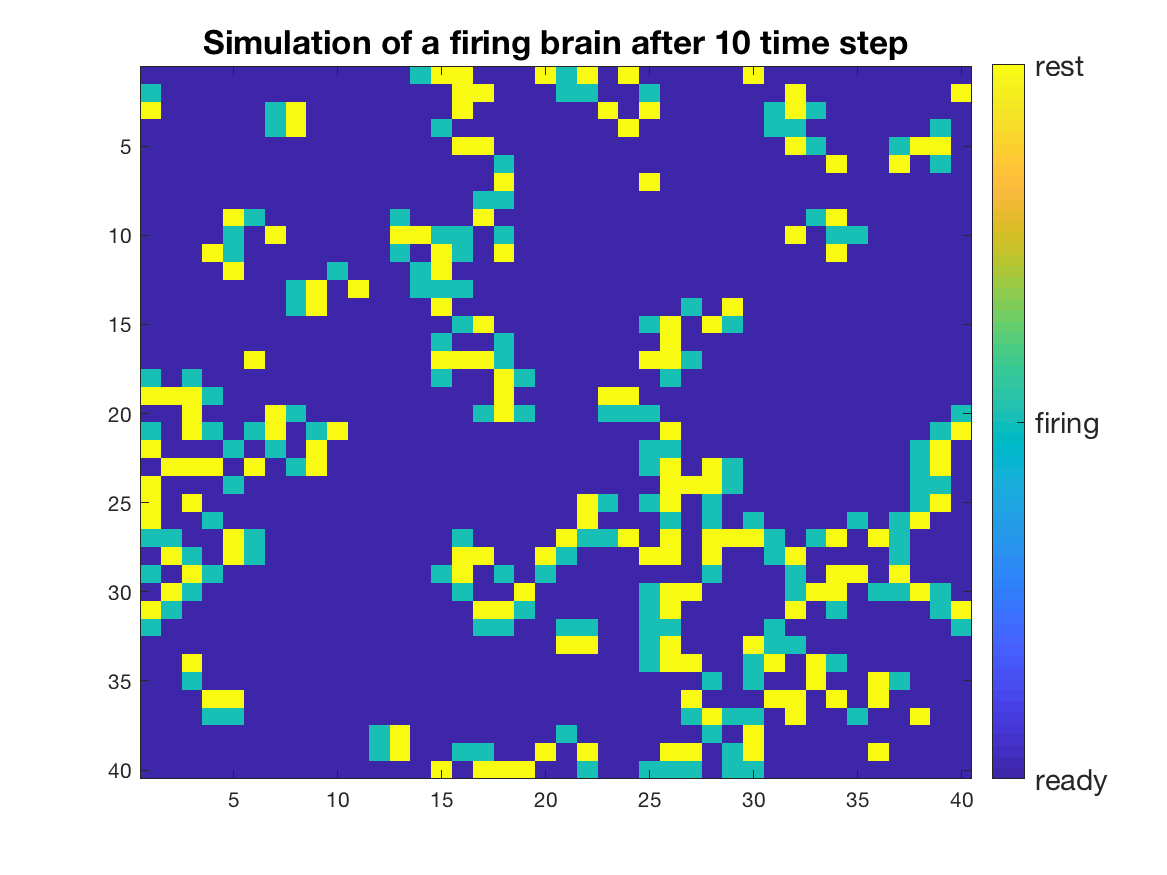
\includegraphics[width = 12 cm, height = 9cm]{fire10.png}
\caption{40x40 cell grid at t = 10}
\label{fig:fire10}
\end{figure}

\begin{figure}[H] %figure 1 at t=20
\centering
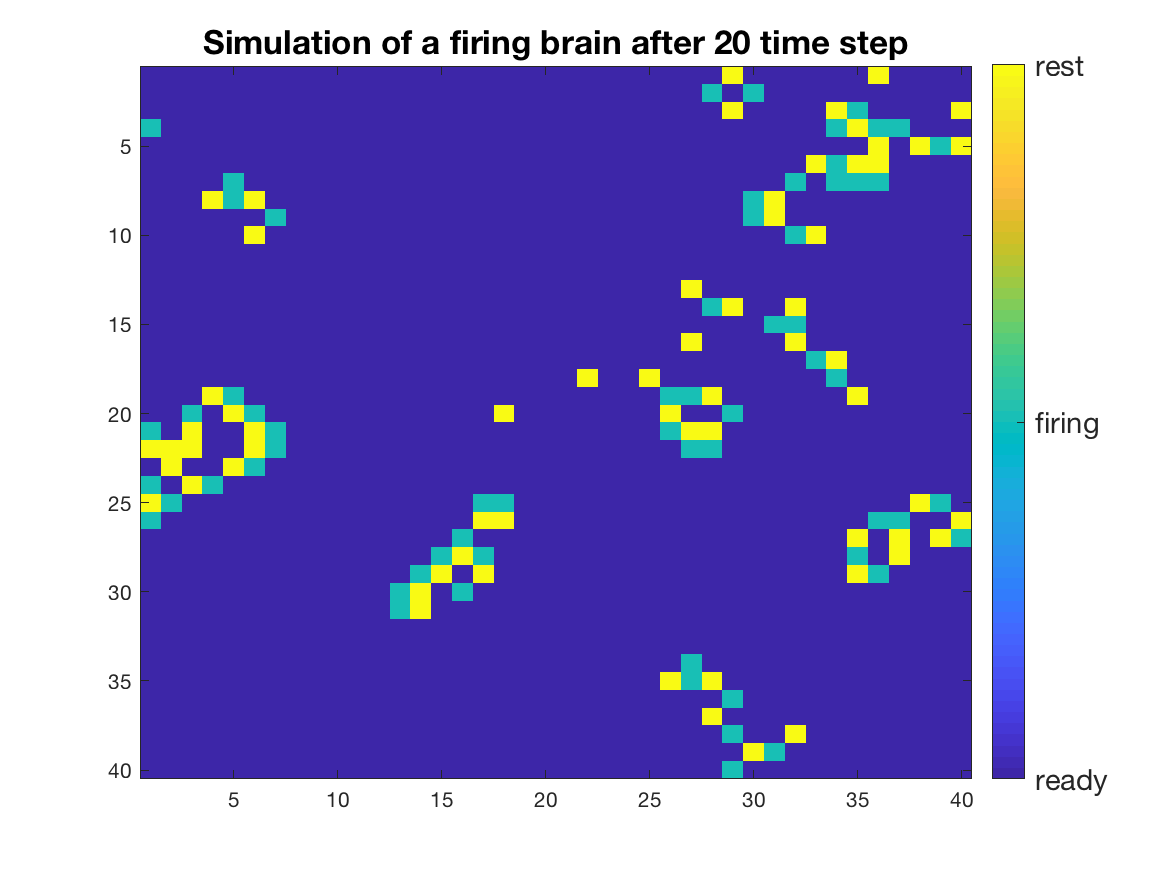
\includegraphics[width = 12 cm, height = 9cm]{fire20.png}
\caption{40x40 cell grid at t = 20}
\label{fig:fire20}
\end{figure}

\begin{figure}[H] %figure 1 at t=100
\centering
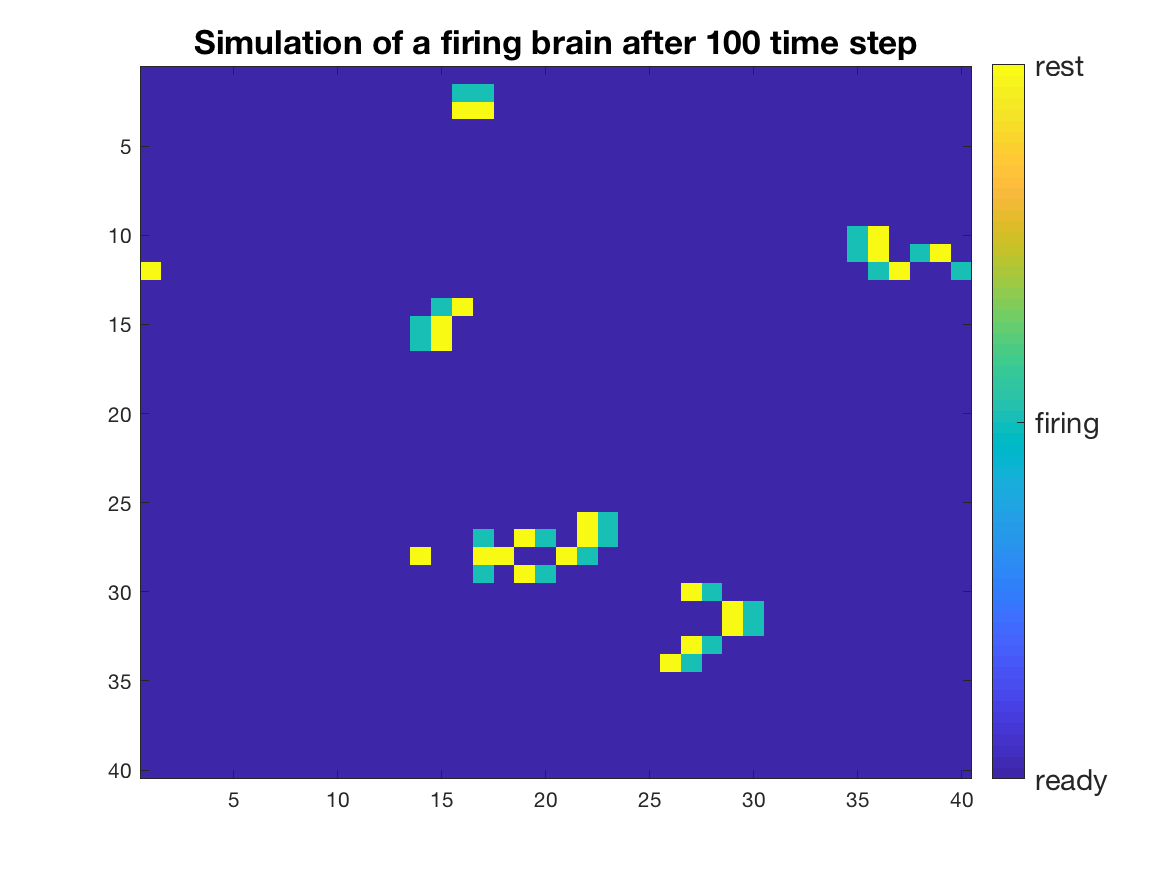
\includegraphics[width = 12 cm, height = 9cm]{fire100.png}
\caption{40x40 cell grid at t = 100}
\label{fig:fire100}
\end{figure}

\begin{figure}[H] %figure 1 at t=1000
\centering
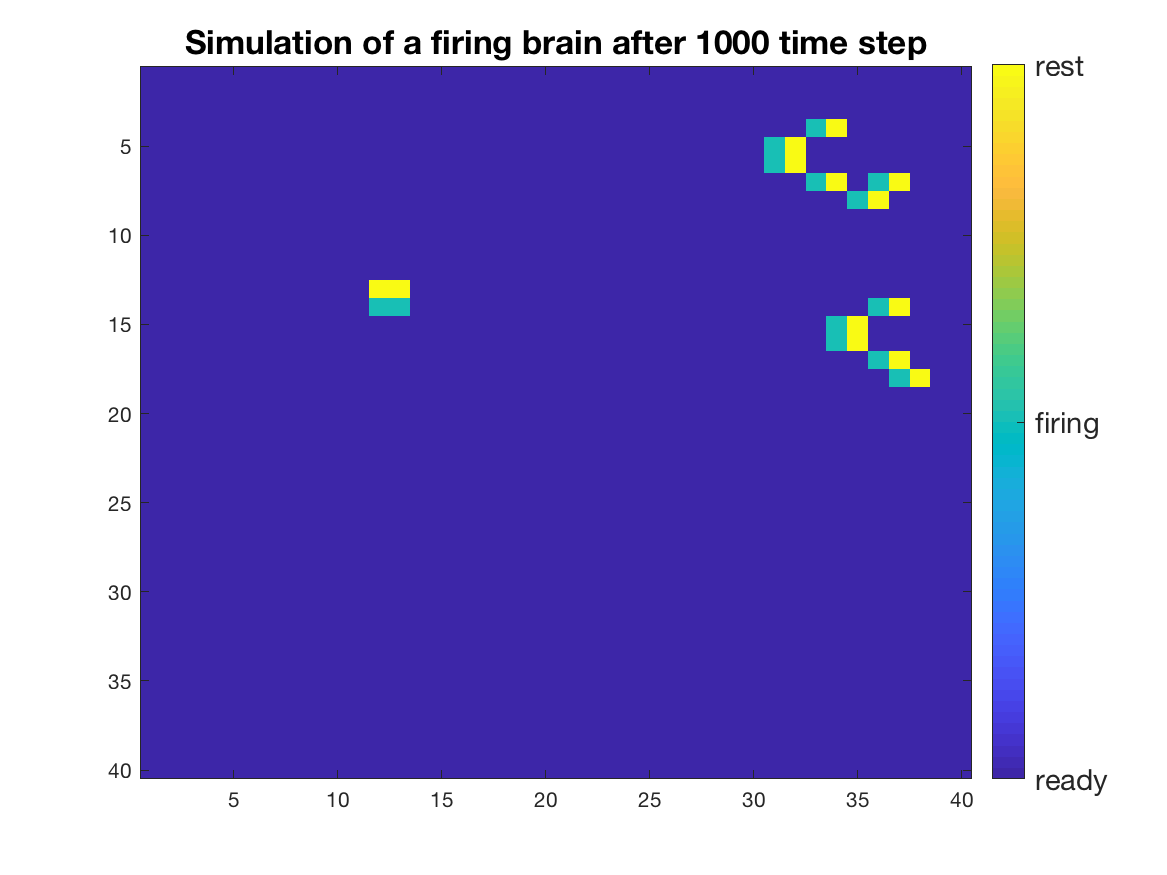
\includegraphics[width = 12 cm, height = 9cm]{fire1000.png}
\caption{40x40 cell grid at t = 1000}
\label{fig:fire1000}
\end{figure}

\begin{figure}[H] %figure 1 at t=1000
\centering
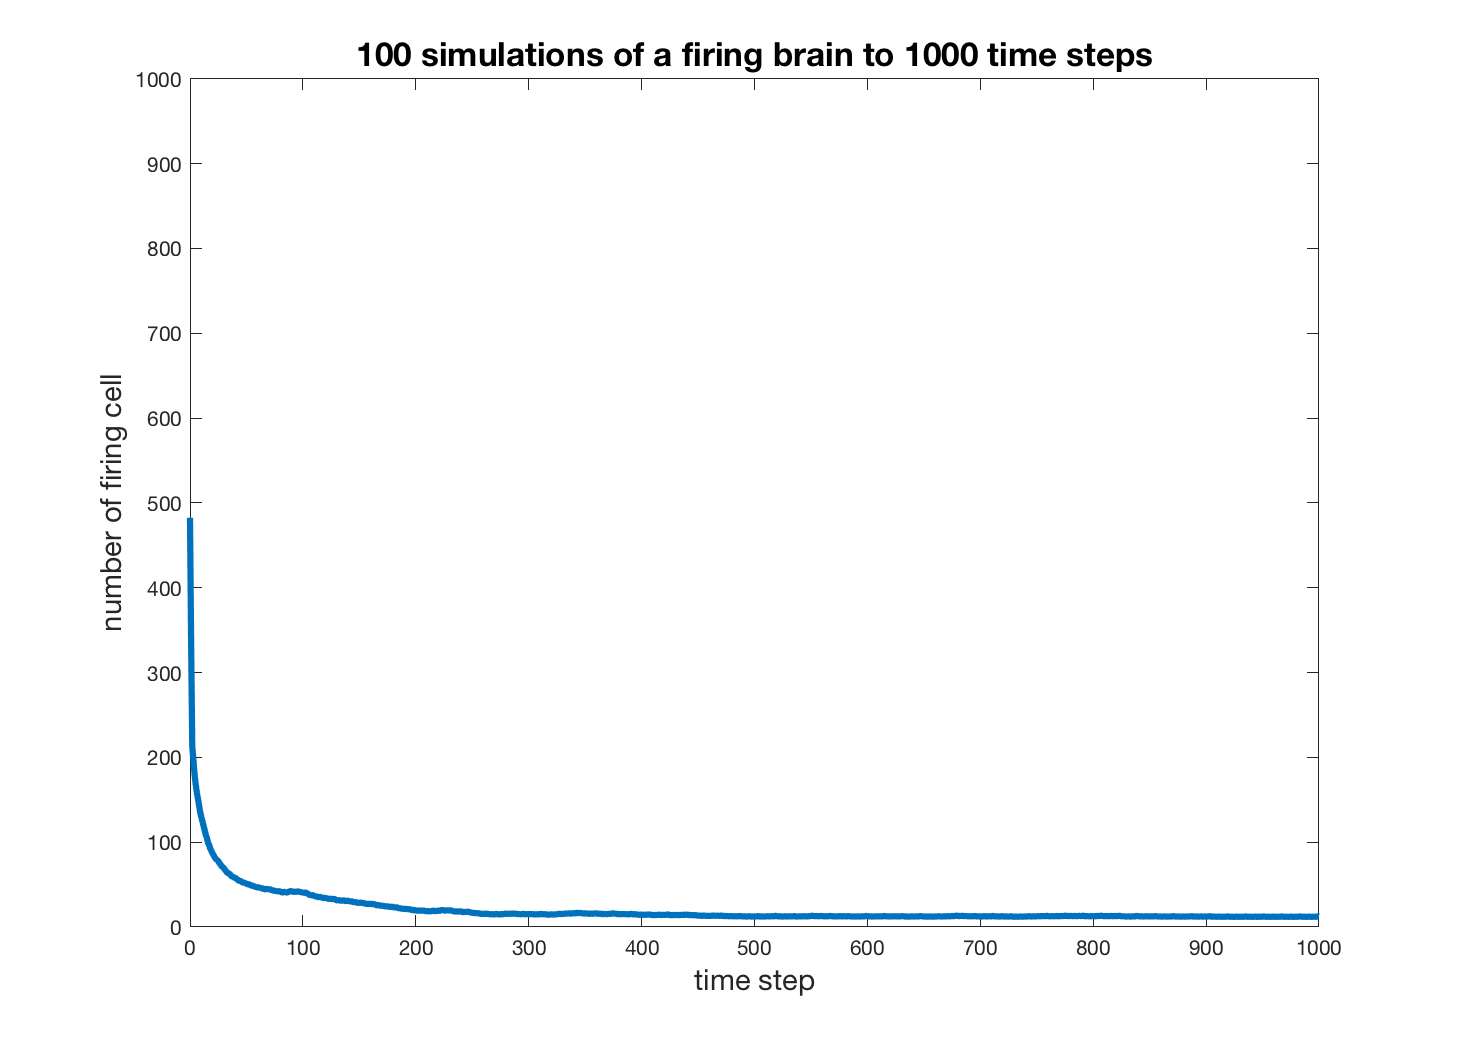
\includegraphics[width = 12 cm, height = 9cm]{firebrain100sim.png}
\caption{average number of firing cells over time with 100 simulation of different initial conditions}
\label{fig:100sim}
\end{figure}

\begin{figure}[H] %model fit
\centering
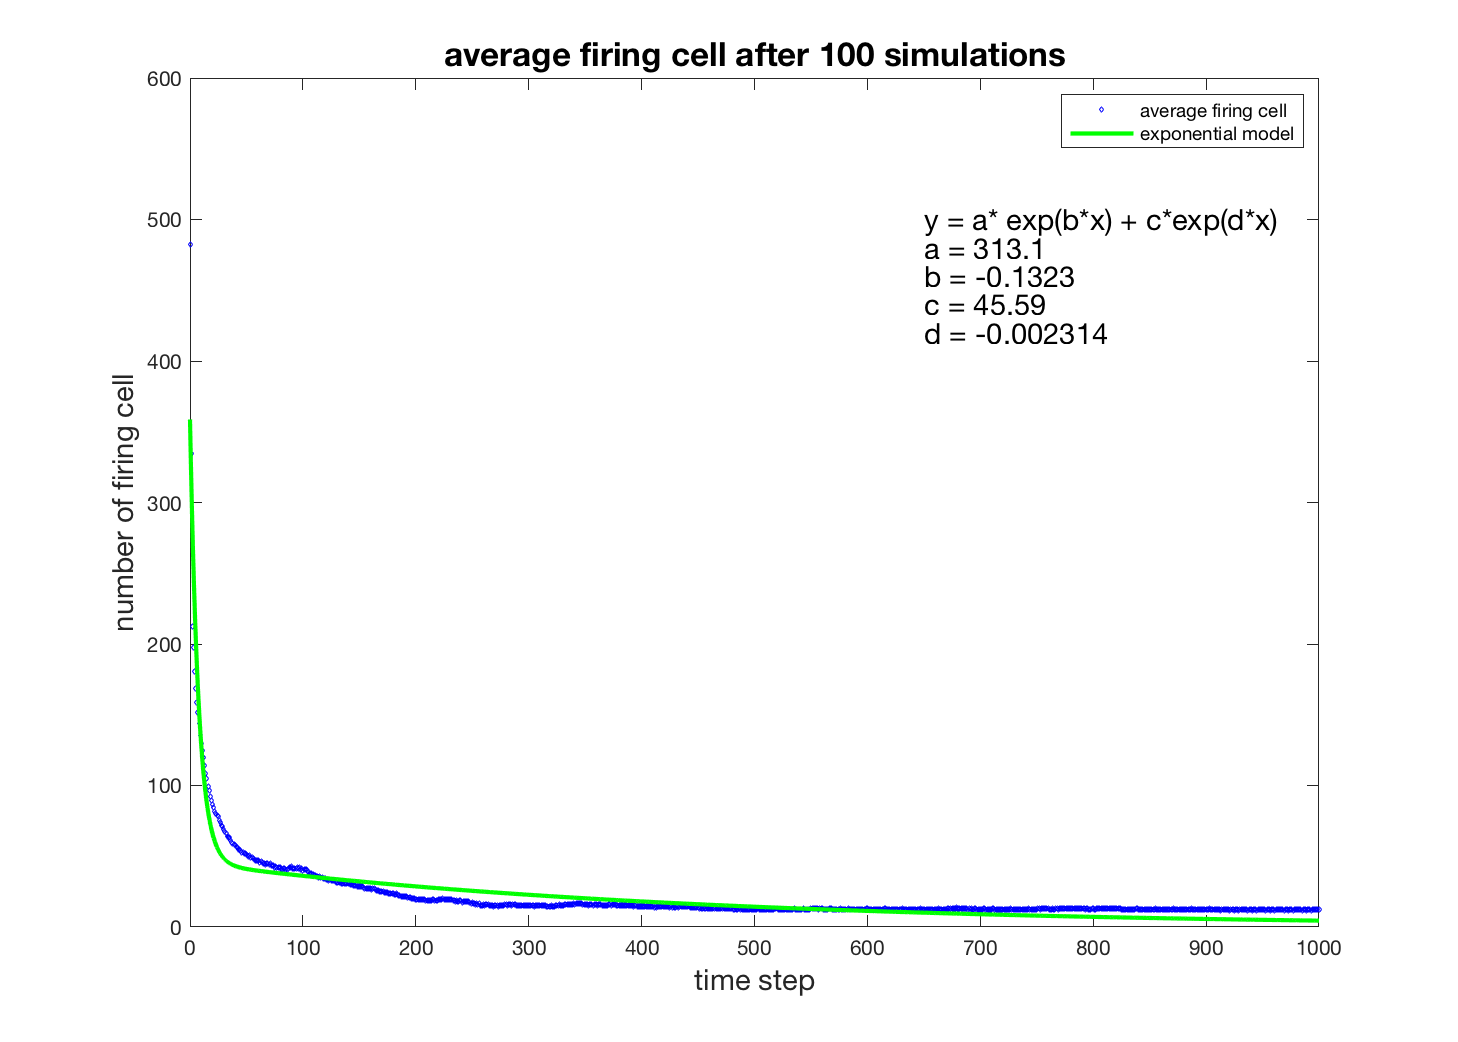
\includegraphics[width = 12 cm, height = 9cm]{sim_model.png}
\caption{average number of firing cells over time with 100 simulation and exponential model fitting}
\label{fig:sim_model}
\end{figure}

%%%%%%%%%%%finish 1.1 %%%%%%%%%%%%


%%%%%%%%%% start 1.2%%%%%%%%%%%%%%

\subsection{example of shapes}

\subsubsection{move forward at a rate of one cell per time step, while preserving the same shape}
\begin{figure}[H] %move forward space ship
\centering
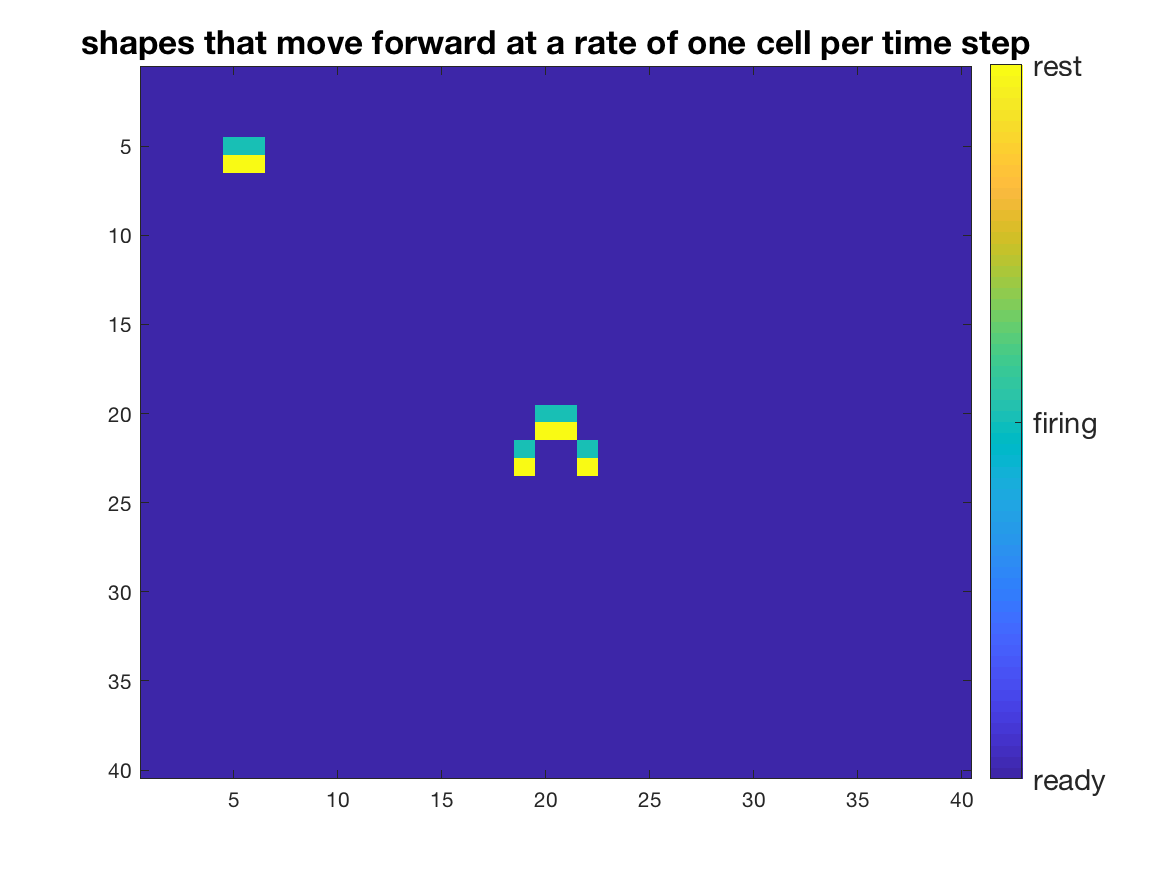
\includegraphics[width = 16 cm, height = 13cm]{task2_1.png}
\caption{shapes that move forward at a rate of one cell per time step preserving the same shape}
\label{fig:task2_1}
\end{figure}

\subsubsection{move forward at a rate of one cell per time step, launching other shapes behind them}
\begin{figure}[H] %launch other shapes
\centering
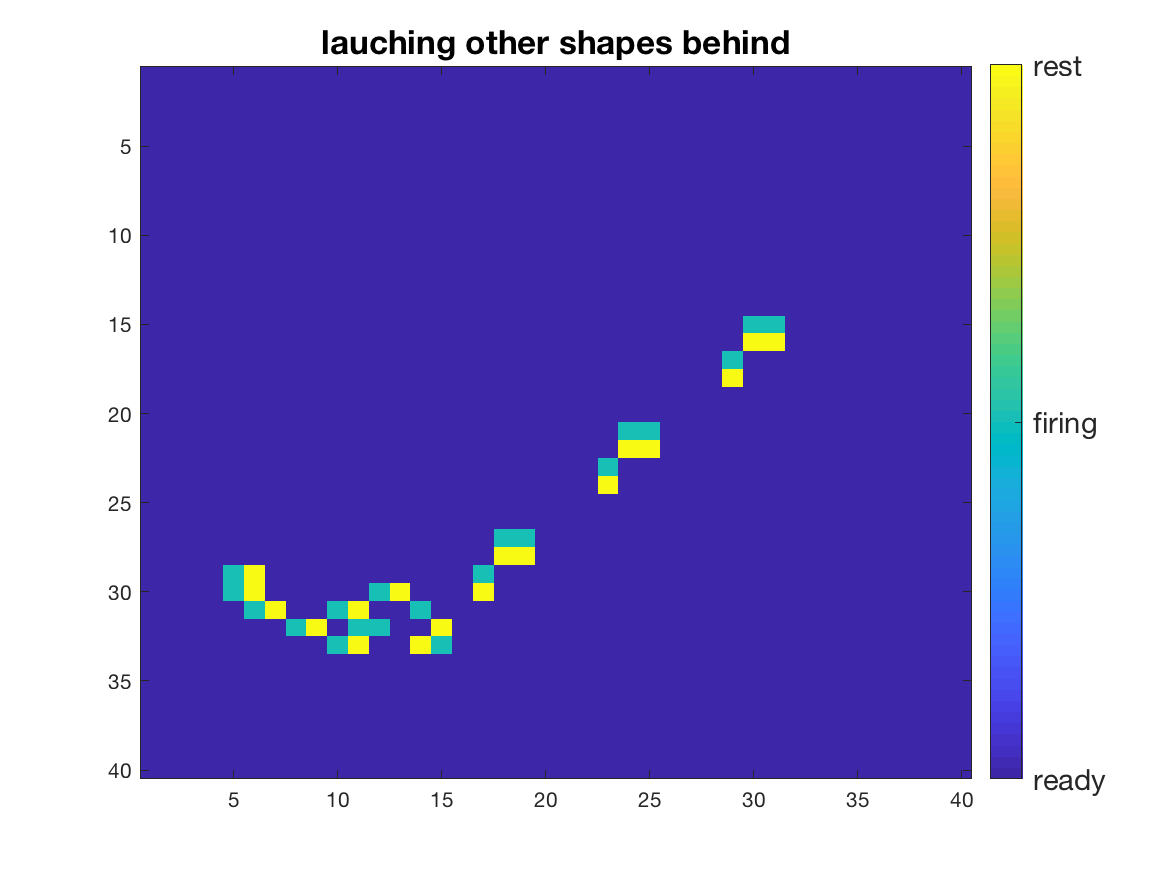
\includegraphics[width = 16 cm, height = 13cm]{task2_2.png}
\caption{shapes that move forward at a rate of one cell per time step, launching other shapes behind them}
\label{fig:task2_2}
\end{figure}

\subsubsection{move forward at a rate of less than one cell per time step, while returning to the same shape after some period}
\begin{figure}[H] %move slower than 1 cell per time
\centering
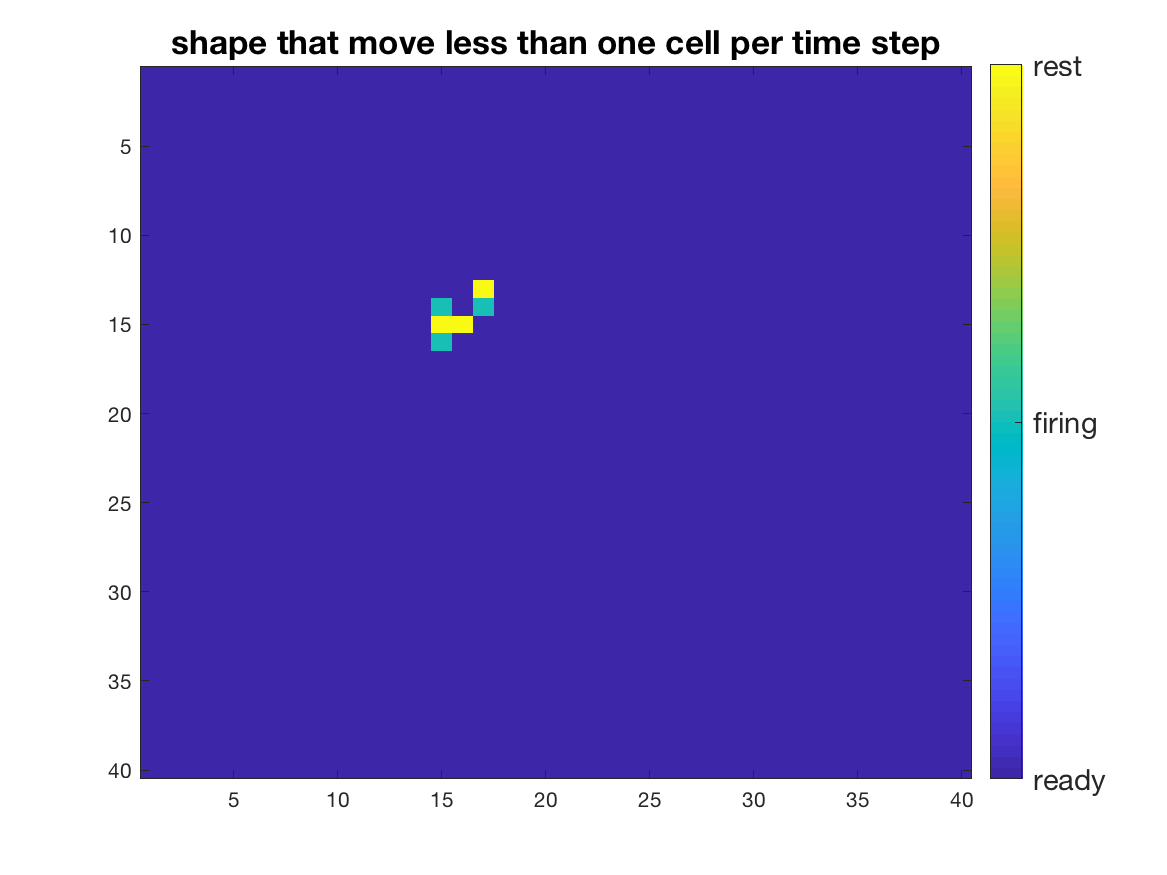
\includegraphics[width = 16 cm, height = 13cm]{task2_3.png}
\caption{shapes that move less than one cell per time step, returning to same shape after some period}
\label{fig:task2_3}
\end{figure}

\subsubsection{stay stationary but oscillate periodically}
\begin{figure}[H] %oscillate
\centering
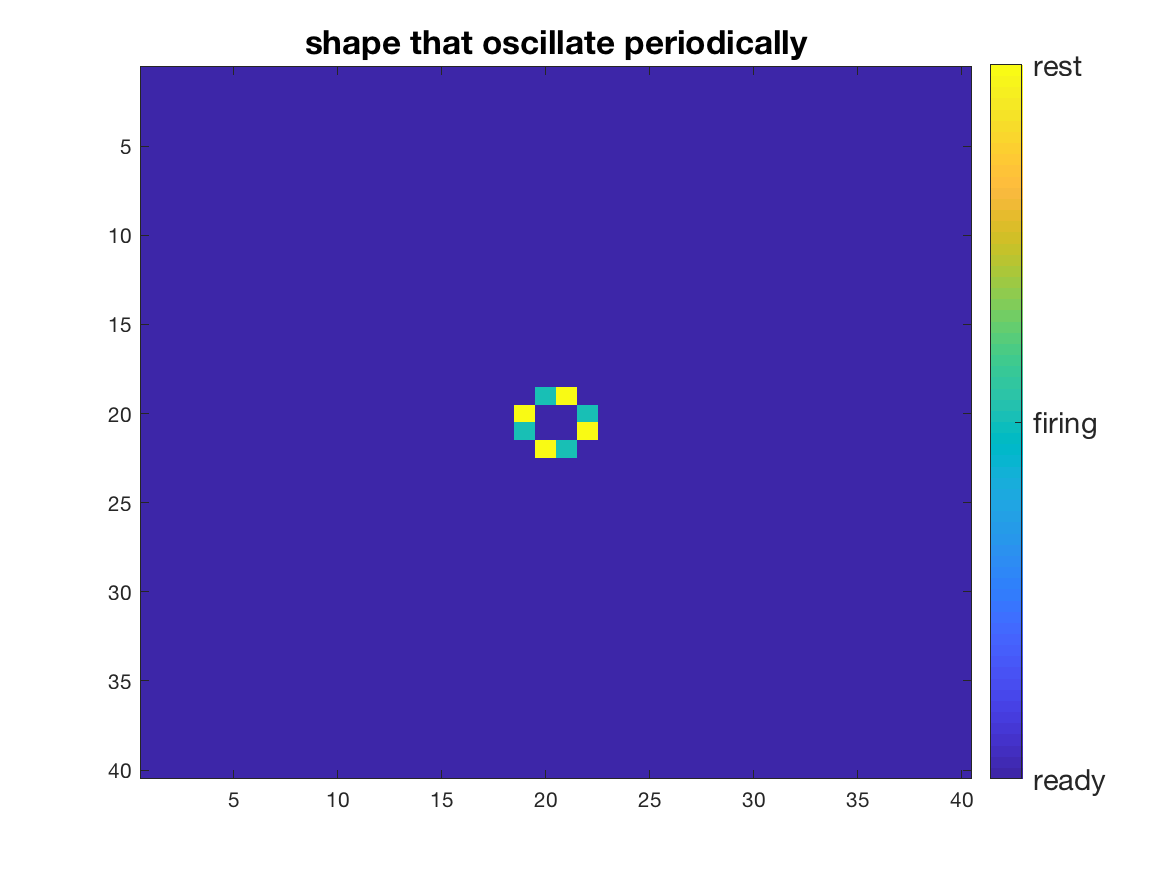
\includegraphics[width = 16 cm, height = 13cm]{task2_4.png}
\caption{shapes that stay stationary but oscillate periodically}
\label{fig:task2_4}
\end{figure}

%%%%%%%%%%%%%end of 1.2

\subsection{create cellular automata}
%%%%%%%leave it as now. 
%%%%%%%%%%%%%%%
%%%%%%%%%%%%%%%

%%%%%%%%%%%%%%%
%%%%%%%%%%%%%%%2. memes
\section{Spread of memes}
\doublespacing
In this part, a model is used to simulate the spread of internet memes. There are 3 different states, resting(0), sharing(1) and bored(2). The rules for the next time step are:

\begin{enumerate}
\item with probability p = 0.001, a person at rest will discover a new meme and become a sharer.(0 $\rightarrow$ 1 with p = 0.001) 
\item with probability q = 0.01, a person sharing(1) will pick one person completely at random from the population to share the memes with. if the random person is at rest(0), that person will become a sharer(1), if that person is bored(2), then the sharing person will become bored(2). 
\item bored(2) stays bored(2) forever. (2 is always 2).
\end{enumerate}

\subsection{some simulations in matlab}
the simluation in matlab will run the model 1000 times with a population of 1000 to time at 2000. and show the change of number of resting, sharing and bored person over time. The initial condition is that there are one person sharing and one bored person. and below are the graphs showing the simulation. 

\begin{figure}[H] %1000 meme run >.<
\centering
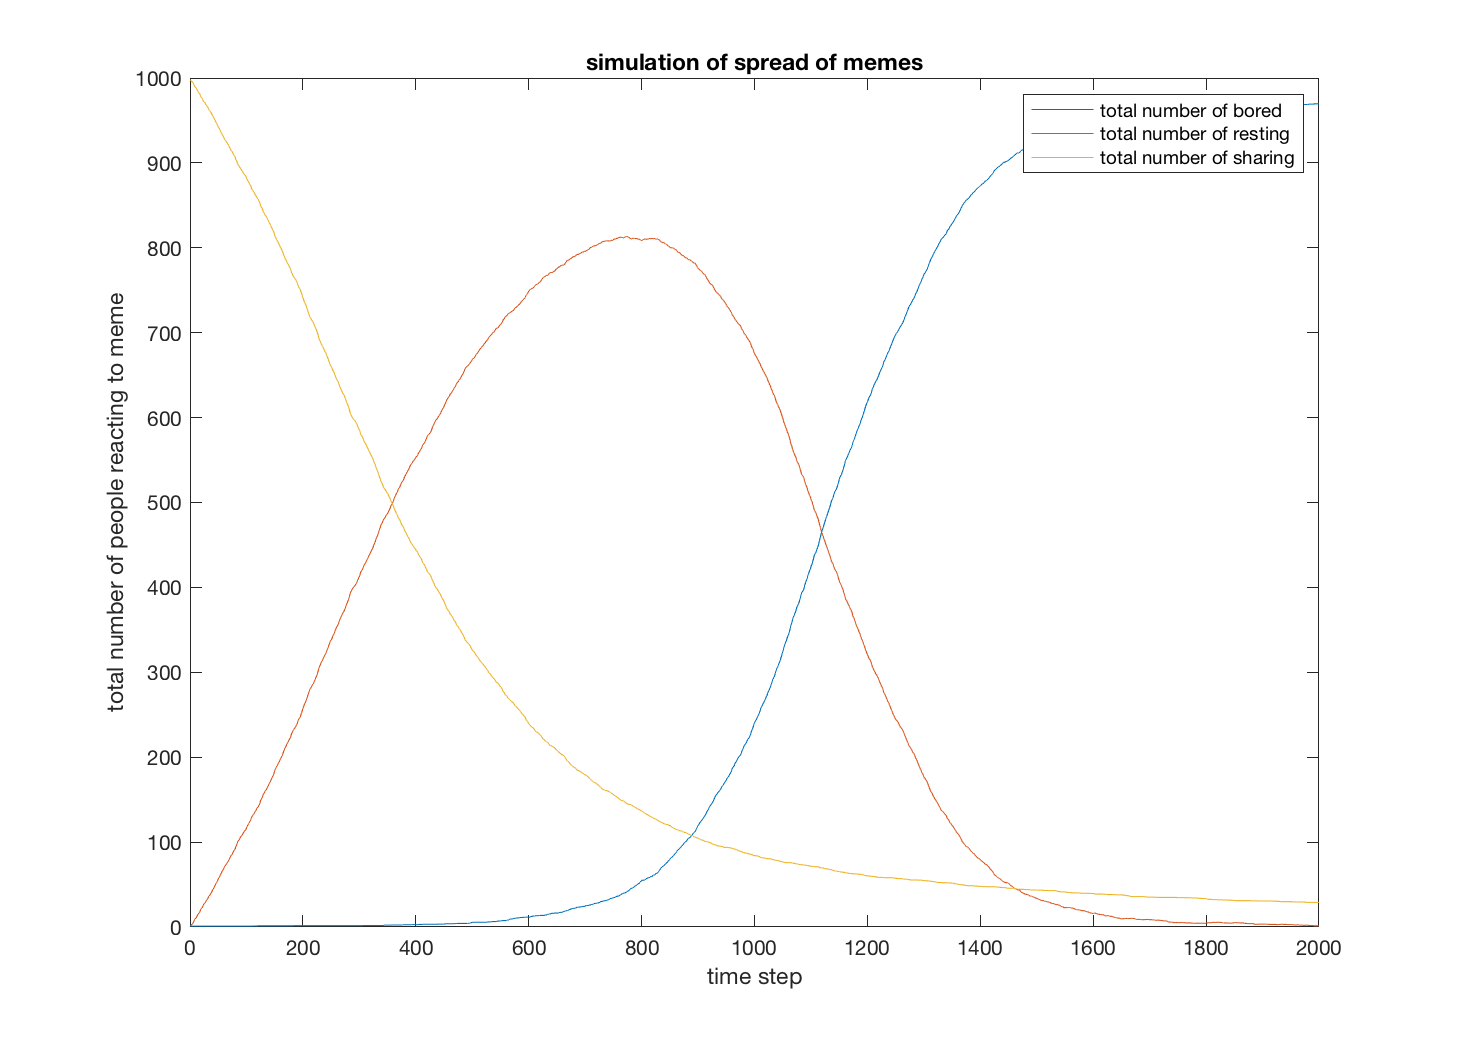
\includegraphics[width = 16 cm, height = 13cm]{memes_1.png}
\caption{simulation of spread of memes showing number of bored, sharing, resting person over time}
\label{fig:meme_sim}
\end{figure}

The difference equation model for the sharing of meme is: 






In matlab, we define a geometry by calling circleg (a unit circle) and then call initmesh to create a mesh with a defined maximum maximum mesh size. the first part of setting up a 2D analysis is by setting up a model for a time-independent problem, here the Laplace operation is $\bigtriangleup = \partial^2\partial x_1^2 + \partial^2/ \partial x_2^2$:
\begin{numcases}{ }
	-\bigtriangleup u(x) = f(x), \quad x \in \textit{B}\\
	u(x) = u_{exact}(x), \quad x \in \partial \textit{B} \\
	f(x) = 8\pi^2 sin(2\pi x_1) sin(2\pi x_2)\\
	u_{exact}(x) = sin(2\pi x_1)sin(2\pi x_2)
\end{numcases}
Here we form the weak form and discrete the domain and use linear algebra to find the approximate solution for u. \par
The weak form: 
\begin{align}
	&-\int_{\Omega} \bigtriangleup uvdx = \int_{\Omega} fv dx \\
	&\int_{\Omega} \bigtriangledown u \cdot \bigtriangledown v dx  - \int_{\partial \Omega} n \cdot \bigtriangledown uvds = \int_{\Omega} fv dx \\
	&\int_{\Omega} \bigtriangledown u \cdot \bigtriangledown v dx = \int_{\Omega} fv dx 
\end{align}
And constructing the stiffness matrix A, mass matrix M and load vector b are similar to the 1D FEM analysis, the details of how to construct the matrix in matlab can be found in the appendix. \par
to solve equation, we use different mesh size: $h_{max} = \{ \frac{1}{2}, \frac{1}{4}, \frac{1}{8}, \frac{1}{16}, \frac{1}{32} \}$. and we will find the convergence rate at around 1.4 from Figure \ref{fig:2d_convergence} which we may conclude that the convergency rate is 1. And we can see the $h_{max}$ vs. $h_{max}^{\gamma}$ with $\gamma = 1.4354$ in Figure \ref{fig:2d_hgamma}.  the solution of the Laplace equation (29) is in Figure \ref{fig:2d_solution}. \par

\begin{figure}[H] %figure 2
\centering
\includegraphics[width = 18 cm, height = 15cm]{energynorm.png}
\caption{2D energy norm with different mesh size}
\label{fig:2d_convergence}
\end{figure}

\begin{figure}[H] %figure 3
\centering
\includegraphics[width = 18 cm, height = 15cm]{hgamma.png}
\caption{$h_{max}$ vs. $h_{max}^{\gamma}$}
\label{fig:2d_hgamma}
\end{figure}

\begin{figure}[H] %figure 4
\centering
\includegraphics[width = 10cm, height = 20cm]{2dsolution.png}
\caption{2D solution with mesh size of $\frac{1}{2}$ and $\frac{1}{32}$}
\label{fig:2d_solution}
\end{figure}

\subsection{2D torus}
In 2D analysis for the torus, we start with a unit circle and set the boundary for torus as equation (5). The derivative in time is $\partial _t u$ is approximated using the Crank-Nicolson method, $k_i$ is the time step: 

\begin{equation}
	M \frac{\xi_i - \xi_{i-1}}{k_i} + A \frac{\xi_i + \xi_{i-1}}{2} = \frac{b_i + b_{i-1}}{2}
\end{equation}

in the system to solve for the the equation, we have the stiffness matrix (A):
\begin{equation}
	A_{ij} = \int_{\Omega} \bigtriangledown \phi _j \cdot \bigtriangledown \phi _i dx
\end{equation}

Mass matrix (M):

\begin{equation}
	M_{ij} = \int_{\Omega}  \phi _i \cdot  \phi _j dx
\end{equation}

Load vector(b):
\begin{equation}
	b_{i} = \int_{\Omega}  f  \phi _i dx
\end{equation}

Boundary matrix (R):
\begin{equation}
	R_{ij} = \int_{\partial \Omega}  \gamma \bigtriangledown \phi _i \cdot  \bigtriangledown \phi _j ds
\end{equation}

Boundary vector (r):
\begin{equation}
	r_{ij} = \int_{\partial \Omega}  \gamma g \phi _i ds
\end{equation}

For the 2D model, we will iterate each element and build the local matrix and vector and map it to the global matrix and vector, the detailed code are in the appendix. The parameters for the torus are: $\rho = 10$, $R = 0.5$, $r = 0.3$, final time = 30. and we use two different mesh size $h_{max} = \frac{1}{5}$ and $h_{max} = \frac{1}{20}$. and the initial state and the final state using both mesh are shown in Figure \ref{fig:2d_fem} and the mass loss computed using $u_{initial} - u_h$ and the mass loss over time is ploted in Figure \ref{fig:2d_massloss}. \par

\begin{figure}[H] %figure 5
\centering
\includegraphics[width = 18 cm, height = 15cm]{torus_2d_solution.png}
\caption{2D torus solution with two different mesh size}
\label{fig:2d_fem}
\end{figure}

\begin{figure}[H] %figure 6
\centering
\includegraphics[width = 10cm, height = 20cm]{torus_2d_hormone_emission.png}
\caption{2D torus hormone emission}
\label{fig:2d_massloss}
\end{figure}


\section{3D model}

\subsection{FEniCS implementation for 2D and 3D mesh}
FEniCS (\url{https://fenicsproject.org/}) is an open source finite element software that can solve partial differential equations in any space dimensions and polynomial degrees. We will implement FEniCS with a 2D mesh for equation (1), (2), (3), and (5) and with the 3D mesh for equation (1), (2), (3), and (4). and the parameters are $\rho = 10$, $R = 0.5$, $r = 0.2$ and $ T = 20$. and the results are plot below. in Figure \ref{fig:2d_t0_fenics} and Figure \ref{fig:2d_t20_fenics}, the visualisation is for the 2D torus at t = 0 and t = 20. in Figure \ref{fig:3d_t0_x} and \ref{fig:3d_t0_z} the 3D torus at t = 0 are plotted along x axis and z axis. and in Figure \ref{fig:3d_t20_x} and Figure \ref{fig:3d_t20_z} are the results at t = 20 for the 3D torus along x axis and z axis. The visualisation for the shape of the torus is in Figure \ref{fig:3d_torus}. \par
The tutorial of implementing FEniCS can be found on the website of the FEniCS and for the torus, the detailed code are in the appendix. \par

\begin{figure}[H] %figure 7 2d torus in fenics t0
\centering
\includegraphics[scale = 0.65]{2d_t0.png}
\caption{2D torus at t = 0 using FEniCS}
\label{fig:2d_t0_fenics}
\end{figure}

\begin{figure}[H] %figure 8 2d torus in fenics t20
\centering
\includegraphics[scale = 0.65]{2d_t20.png}
\caption{2D torus at t = 20 using FEniCS}
\label{fig:2d_t20_fenics}
\end{figure}

\begin{figure}[H] %figure 9 3d torus in fenics t0
\centering
\includegraphics[scale = 0.65]{3d_t0_1.png}
\caption{3D torus at t = 0 along the x axis using FEniCS}
\label{fig:3d_t0_x}
\end{figure}

\begin{figure}[H] %figure 10 3d torus z axia
\centering
\includegraphics[scale = 0.65]{3d_t0_1z.png}
\caption{3D torus at t = 20 along the z axis using FEniCS}
\label{fig:3d_t0_z}
\end{figure}

\begin{figure}[H] %figure 11 3d torus in fenics t20
\centering
\includegraphics[scale = 0.65]{3d_t20_1.png}
\caption{3D torus at t = 20 along the x axis using FEniCS}
\label{fig:3d_t20_x}
\end{figure}

\begin{figure}[H] %figure 12 3d torus in fenics t20 z axis
\centering
\includegraphics[scale = 0.65]{3d_t20_1z.png}
\caption{3D torus at t = 20 along the z axis using FEniCS}
\label{fig:3d_t20_z}
\end{figure}

\begin{figure}[H] %figure 13 3d torus view 
\centering
\includegraphics[scale = 0.65]{3d_torus_sphere.png}
\caption{3D torus view}
\label{fig:3d_torus}
\end{figure}


\subsection{3D torus hormone emission analysis}

In order to compute the hormone emission from the torus, we can treat the hormone emission as mass loss, at each time level, we compute the mass loss inside the while loop for computing solution at each time step and save it to a file. in this part, we used the mesh sphere1.xml. 
\begin{align}
	&M = (u_{initial} - u)*dx\\
	&mass = assemble(M)
\end{align}
Here three different sets of control parameters are tested and the mass loss are plot in the same figure. the parameters are:
\begin{align}
	&\rho = 10, R = 0.5, r = 0.2, T = 50\\
	&\rho = 20, R = 0.5, r = 0.2, T = 50\\
	&\rho = 40, R = 0.5, r = 0.2, T = 50
\end{align}
and the results using two different mesh sphere1 and sphere2 are plot separately in Figure \ref{fig:mass_loss1} and Figure \ref{fig:mass_loss2}. as we can see from both figures, setting a higher $\rho$ will result in a faster mass loss. The equation for the torus is in diffusion. Over time, the hormone inside the torus will diffuse very fast in the beginning and then the speed of mass loss will slow down and get very close to 0 at $t_{end}$. and the larger the source term ($\rho$), the faster the mass loss.  
\begin{figure}[H] %figure 14 mass loss for torus 
\centering
\includegraphics[scale = 0.6]{mass_loss_mesh1.png}
\caption{Torus mass loss with different $\rho$ using mesh sphere1.xml}
\label{fig:mass_loss1}
\end{figure}

\begin{figure}[H] %figure 14 mass loss for torus 
\centering
\includegraphics[scale = 0.6]{mass_loss_mesh2.png}
\caption{Torus mass loss with different $\rho$ using mesh sphere2.xml}
\label{fig:mass_loss2}
\end{figure}
\newpage
\subsection{Torus optimisation}
The last part of designing the torus is that the torus will need to achieve at time $t = \{ 5, 7, 30\} $ dose amount $M = \{10, 15, 30 \}$ mmol. Using scipy.optimize, and we compute the error of target dose at $t = \{ 5, 7, 30\} $ and the actual dose. with initial data of $[\rho, R, r]$ at $[20, 0.5, 0.1]$, we get the optimised result of the torus at $[40.9, 0.5, 0.3]$. 
\\[1cm]

\section{Conclusion}
In this project, a medical torus is designed step by step from 1D to 2D and then 3D with optimised dosage. the optimised torus have the following data $[\rho, R, r]$: $[40.9, 0.5, 0.3]$.\\
\newpage


\section{Reference}

\begin{enumerate}
\item Larson, M., Bengzon, F., 2013, Ume\aa, The Finite Element Methods: Theory Implementation and Applications.
\item Nazarov, M., 2017, Uppsala,  Applied Finite Element Course material
\end{enumerate}


\section{Appendix}

\subsection{1D code in matlab}
\singlespacing
\begin{itemize}
\item {\large my{\_}stiffness{\_}matrix{\_}assembler.m}
\lstinputlisting{my_stiffness_matrix_assembler.m}
\vspace{1cm}

\item {\large my{\_}load{\_}vector{\_}assembler.m}
\lstinputlisting{my_load_vector_assembler.m}
\vspace{1cm}

\item {\large laplacian.m}
\lstinputlisting{laplacian.m}
\vspace{1cm}

\item {\large errorest.m}
\lstinputlisting{errorest.m}
\vspace{1cm}

\item {\large f.m}
\lstinputlisting{f.m}
\vspace{1cm}

\item {\large my{\_}fem{\_}solver.m}
\lstinputlisting{my_fem_solver.m}
\vspace{1cm}
\end{itemize}

\subsection{2D code in matlab}
\doublespacing
\subsubsection{2D time independent Laplace equation code in matlab}

\singlespacing
\begin{itemize}

\item{\large my2dsolver.m}
\lstinputlisting{my2dsolver.m}
\vspace{1cm}

\item{\large assemble.m}
\lstinputlisting{assemble.m}
\vspace{1cm}

\item{\large f1.m}
\lstinputlisting{f1.m}
\vspace{1cm}
\item{\large g1.m}
\lstinputlisting{g1.m}
\vspace{1cm}

\end{itemize}


\subsubsection{2D torus code in matlab}

\singlespacing
\begin{itemize}

\item{\large partB{\_}2d{\_}torus.m}
\lstinputlisting{partB_2d_torus.m}
\vspace{1cm}

\item{\large assemble.m}
\lstinputlisting{assemble.m}
\vspace{1cm}

\item{\large torus{\_}2d.m}
\lstinputlisting{torus_2d.m}
\vspace{1cm}

\item{\large mass{\_}loss.m}
\lstinputlisting{mass_loss.m}
\vspace{1cm}

\item{\large f2.m}
\lstinputlisting{f2.m}
\vspace{1cm}

\item{\large g.m}
\lstinputlisting{g.m}
\vspace{1cm}

\end{itemize}

\subsection{3D code in python implement FEniCS}
\singlespacing
\begin{itemize}

\item{\large projectc1{\_}2d.py}
\lstinputlisting{projectc1_2d.py}
\vspace{1cm}

\item{\large projectc1{\_}3d.py}
\lstinputlisting{projectc1_3d.py}
\vspace{1cm}

\item{\large projectc2{\_}3d.py}
\lstinputlisting{projectc2_3d.py}
\vspace{1cm}

\item{\large c2{\_}mass{\_}plot.py}
\lstinputlisting{c2_mass_plot.py}
\vspace{1cm}

\item{\large projectc3{\_}optimization.py}
\lstinputlisting{projectc3_optimization.py}
\vspace{1cm}


\end{itemize}


\end{document}